\documentclass[14pt,a4paper,onecolumn]{article}
\usepackage[utf8]{inputenc}
\usepackage{amsmath}
\usepackage{amsfonts}
\usepackage{amssymb}
\usepackage{graphicx}
\usepackage{natbib}


\bibliographystyle{apalike}
\setlength{\parskip}{1.2em}
\setlength{\parindent}{0pt}
% \graphicspath{{./images/}}

\author{Ibrahim AbuBakr ElSeddiq}
\title{The predictive value of NTproBNP on postoperative outcome in patients undergoing offpump CABG}

\begin{document}

\maketitle

\tableofcontents
\clearpage

\listoffigures
\clearpage

\listoftables
\clearpage

\section{Introduction}

Coronary heart disease is the main cause of morbidity and mortality in developed countries, and the prevalence is increasing in developing countries.  Several studies have reported biomarker clusters which are associated with CHD.  The assessment of these biomarkers, alone or in combination, may improve the long-term prediction of mortality of first major cardiovascular event compared to conventional risk markers. \citep{Zetheliusetal2008}

Brain type natriuretic peptide (BNP) is primarily produced by cardiac myocytes. Physiological effects of BNP are a peripheral vasodilatation and inhibition of renin-angiotensin production. \citep{DanielsandMaisel2007} The precursor peptide proBNP is split into the active hormone BNP and the N-terminal fragment (NT-proBNP).  Both BNP and NT-proBNP are established markers for cardiac failure.  NT-proBNP is also more stable, which makes its measurement more reliable. \citep{Thay-Hsiungetal2013} NT-proBNP was identified as a novel and important CHD biomarker, and has prognostic value in patients with stable CHD. \citep{Kragelundetal2005} A report from the BELSTRESS study suggested that NT-proBNP levels were a strong predictor of coronary events, even after adjustment for conventional risk factors. \citep{DeSutteretal2005} In patients with coronary artery disease increased BNP levels are associated with an increased  rate of myocardial infarction and cardiovascular death during mid-term follow-up. \citep{Schabeletal2006}

However, Other pathologies such as exacerbated chronic obstructive pulmonary disease, atrial fibrillation, and myocarditis can cause elevated BNP levels. Additionally, higher NT-proBNP levels are associated with : female gender, impaired renal fuction, and older age.  Increased BNP levels are a prognostic marker associated with higher mortality in patients with myocardial infarction, cardiogenic shock, and pulmonary embolism. \citep{Rodseth2009}

\section{Review of Literature}

\subsection{Natriuretic Peptides}


\subsubsection{Atrial Natriuretic Peptide}
Since 1956, Kisch found secretory granules in the guinea pig atrium; the heart is recognized not only as the pump of the circulatory system but also an endocrine organ.\citep{Kisch1956} \citep{deBold1979} de Bold and colleagues in Kingston, Ontario, Canada found that rat atrial extracts contained a substance that increased salt and urine output in the kidney.\citep{deBoldetal1981} Later, the substance was purified from the heart by several groups and named ANF or ANP.\citep{deBold1985}  Brain natriuretic peptide was identified from the porcine brain tissue initially and was found primarily synthesized from the ventricle. The name was subsequently changed to B-type natriuretic peptide (BNP). C-type natriuretic peptide (CNP) is produced by vascular endothelial cells and the kidney and is structurally similar to ANP and BNP.

ANP is a 28-amino acid peptide with a 17-amino acid ring in the middle of the molecule. The ring is formed by a disulfide bond between two cysteine residues at positions 7 and 23. ANP is closely related to BNP (brain natriuretic peptide) and CNP (C-type natriuretic peptide), which all share a similar amino acid ring structure.

Human ANP is encoded by the NPPA gene on the short arm of chromosome 1, which has 3 exons and 2 introns. The gene is expressed primarily in cardiac myocytes. Lower levels of NPPA expression are found in other tissues such as the brain, kidney, lung, uterus and placenta.

In cardiac myocytes, ANP is made as a precursor form, i.e. prepro-ANP, a polypeptide of 151 amino acids. After the signal peptide is removed in the endoplasmic reticulum, the 126-amino-acid pro-ANP is stored in the intracellular granules. When the cells are stimulated, pro-ANP is released and converted to the 28-amino-acid C-terminal mature ANP on the cell surface by the cardiac transmembrane serine protease corin.\citep{Yanetal1999}\citep{Yanetal2000}

ANP is secreted in response to:
    \begin{itemize}
        \item Stretching of the atrial wall \citep{Widmaieretal2008}
        \item Reduced Sympathetic stimulation of $\beta$-adrenoceptors
        \item Raised sodium concentration (hypernatremia), though sodium concentration is not the direct stimulus for increased ANP secretion. \citep{Widmaieretal2008}
        \item Endothelin, a potent vasoconstrictor
        \item exercise \citep{Kokkonenetal2002}
    \end{itemize}

BNP can be produced in both atria and ventricles, and is upregulated in failing ventricular myocardium. In response to increased myocardial stretch and wall stress, ventricular myocytes secret the pro-hormone pre-proBNP, which is then cleaved into biologically active BNP and the inactive byproduct N-terminal-proBNP (NT-proBNP). The biological actions of NPs are mediated through membrane-bound natriuretic peptide receptors (NPR) that are linked to a cyclic guanosine monophosphate-dependent signaling cascade, including NPR-A, which preferentially binds ANP and BNP, and NPR-B, which preferentially binds CNP. Elevated BNP levels have been demonstrated to responsed to increased angiotensin II and sympathetic tones. \citep{Iwanagaetal2006}

Elevated NPs levels can be also found in many circumstances involving LV dysfunction or hypertrophy; right ventricular (RV) dysfunction secondary to pulmonary diseases; cardiac inflammatory or infectious diseases; and endocrinology diseases and high output status without decreased left ventricular ejection fraction (EF), e.g., sepsis, renal failure, cirrhosis of liver, or intracranial pathologies. Even in the absence of significant clinical evidence of volume overload or LV dysfunction, markedly elevated NP levels can be found in patients with multiple comorbidities with certain degree of prognostic value. 6 The causes and mechanisms of elevated NPs levels are summarized in Fig. \ref{NP_causes}. The potential clinical applications in the non-HF settings are summarized in Table \ref{NP_applications}.

\begin{figure}
    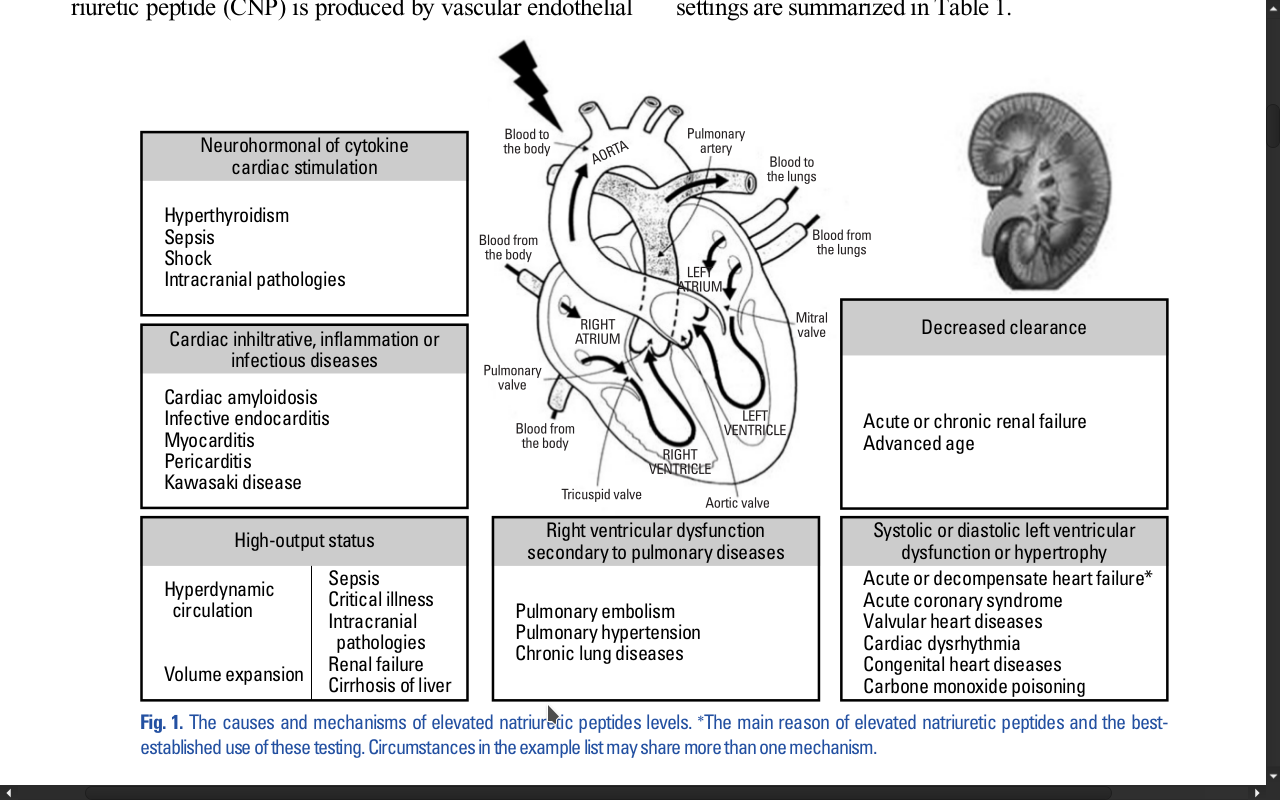
\includegraphics{./images/NP_causes.png}
    \caption{The causes and mechanisms of elevated natriuretic peptides levels. The main reason of elevated natriuretic peptides and the best established use of these testing. Circumstances in the example list may share more than one mechanism.}
    \label{NP_causes}
\end{figure}

\begin{table}
    \begin{tabular}{|l|c|c|c|}
        \hline
        Diseases & Screening &  & Prognosis \\
        \hline
        Heart failure & + & + & + \\
        Acute coronary syndrome & + & + & + \\
        Cardiac procedures & + & + & + \\
        Pulmonary embolism & + & + & + \\
        Pulmonary hypertension & + & + & - \\
        Chronic lung diseases & + & + & + \\
        Valvular heart diseases & + & + & N/A \\
        Cardiac dysrhythmia & + & + & +/- \\
        Cardiac inflammatory or infectious diseases & + & + & N/A \\
        Cardiogenic syncope & + & N/A & N/A \\
        Sleep apnea & + & + & N/A \\
        Hypertension & + & + & N/A \\
        Sepsis & + & + & + \\
        Renal failure & + & + & + \\
        Cirrhosis of liver & + & + & + \\
        Hyperthyroidism & + & + & N/A \\
        Intracranial pathologies & + & + & + \\
        Epilepsy / Seizures & + & - & - \\
        Carbone monoxide poisoning & + & N/A & N/A \\
        \hline
    \end{tabular}
    \caption{Potential Clinical Applications of Natriuretic Peptides in Selected Diseases}
    \label{NP_applications}
\end{table}

\subsection{Coronary Artery Disease}
An extremely short chapter.  No time to be wasted on it.

\subsection{Coronary Artery Bypass Grafting}
Also short
\subsubsection{on-pump vs OPCAB}


\section{Methodology}

\subsection{Population of Study}

Adult patients with coronary artery disease

\subsubsection{Inclusion criteria}

Patients registered for elective OPCAB

\subsubsection{Exclusion criteria}

Patients with signicant valvular heart disease, dilated or hypertophic cardiomyopathy, NYHA III or IV, EF $< 40$, preoperative atrial fibrillation, inotropic support or intra-aortic balloon pump, creatinine clearance $< 60 ml/min/1.73 m^2$, hyperthyoidism and hypothyroidism, and moderate to severe COPD will be excluded to eliminate potential confounding factors which may influence heart function and plasma biomarkers.  Moderate to severe COPD is defined as shortness of breath at own pace on the level, FEV1 $< 80$ of predicted, or continuous use of bronchodilators for $> 2$ weeks.  Hyperthyroidism and hypothyroidism are defined as serum TSH levels outside reference ranges.  It will be measured only upon clinical suspicion.

\subsection{Methodology in details}

60 cases registered for elective off-pump coronary artery bypass grafting OPCAB were recruited in this study. Patients were interviewed preoperatively for history taking and clinical examination. EuroScore II was calculated. Demographic, past medical and surgical history, medications and baseline laboratory results (labs. on admission to hopsital) and preoperative angiography results were recorded.  No specific attempts were made to standardize the aneshetic and surgical management.  Venous samples for measuring NT-proBNP were collected before induction. Samples were sent for analysis in Cairo University Clinical Pathology department. Intra-operative and postoperative data were recorded, including: duration of surgery, number of grafts, intraoperative blood transfusion and, in case CPB was need arotic cross clamp time, CPB time : lowest naso-pharyngeal temp on CPB.Patients were followed during their in-hospital stay and events recorded including: death from cardiovascular causes ischemic stroke (defined as new neurologic deficit lasting for  24hours with definite image evidence of cerebrovascular accident by computed tomography)low output heart failure (defined as need of any of the following: CPB during off-pump surgery, return to CPB after initial separation, intra-aortic balloon pump, inotropes at 48 hours post-operatively) myocardial infarction (defined as elevated tropoponin 10x99th percentile URL at 12 hours after surgery associated with characteristic ECG changes or echocardiographically documented new regional wall motion abnormality). prolonged intubaton  24 hours postoperatively and reintubation arrhythmias.  Statistical package for Social Studies program will be used in the statistical analysis. Numerical data will be expressed as mean, SD and range. Comparisons will be performed by unpaired t test. Categorical variables will be expressed as percentages and compared by chi square test. Correlations will be tested by Pearson's test. P  0.05 is set as statistically significant.

Primary outcomes:
    \begin{itemize}
        \item low output heart failure and myocardial infarction
    \end{itemize}

Secondary outcome parameters:
    \begin{itemize}
        \item moratlity
        \item arrhythmias
        \item length of ICU and in-hospital stay
        \item prolonged intubation
    \end{itemize}


\section{Results}

\section{Discussion}

\section{Conclusion}

\section{Summary}

\newpage

\bibliography{thesis}

\end{document}
